\documentclass[11pt,spanish]{article} % Tipo y tamaño de letra del documento.


\usepackage[utf8]{inputenc}
\usepackage{subfiles}
\usepackage{biblatex}
\addbibresource{references.bib}
\usepackage{multicol}
\usepackage{amsfonts}
\usepackage{blindtext}
\usepackage{mathrsfs}
\usepackage{amsmath}
\usepackage{siunitx}
\usepackage{centernot}
\usepackage[shortlabels]{enumitem}
\usepackage{subfig}
\usepackage{datetime}
\usepackage{listingsutf8}
\usepackage[spanish]{babel}
\usepackage{tikz}
\usepackage{hyperref}
\usepackage[vlined,ruled,linesnumbered]{algorithm2e}
\usepackage{listings}
\usepackage{float}
\usepackage{url}
\usepackage{csquotes}
\usepackage{fourier} %font
\usepackage[top=2cm, bottom=2cm, left=2.5cm, right=2.5cm]{geometry}
\usepackage{pgfplots}
\usepackage{fancyhdr}
\usepackage{mdframed}
\usepackage{tikzducks}
\usepackage[nameinlink]{cleveref}
\usepackage{epigraph} 

\pgfplotsset{compat=1.18}

\usetikzlibrary{shapes.arrows, shapes.geometric, arrows.meta,angles,quotes,positioning,arrows,fit,quotes,calc}
\tikzset{>=latex} 

\setlength\algomargin{1em} 
\SetFuncSty{sc} 
\SetCommentSty{em} 


\Crefname{figure}{Fig.}{Figs.}
\newcommand\crefrangeconjunction{--}
\Crefname{table}{Tabla}{Tablas}
\Crefname{subsubsection}{Subsubsec.}{Subsubsections}
\Crefname{subsection}{Subsec.}{Subsections}
\Crefname{section}{Sec.}{Sections}
\Crefname{equation}{eq.}{eqs.}
\crefname{thm}{Theorem}{theorems}
\Crefname{thm}{Theorem}{Theorems} 

\definecolor{algoco}{rgb}{0,0.4,1}

\hypersetup{
  colorlinks=true,
  linkcolor=algoco,
  citecolor=blue,
  urlcolor=blue,
}

\lstset{
extendedchars=true
inputencoding=utf8/latin1,
basicstyle=\footnotesize\sffamily\color{black},
commentstyle=\slshape \color{gray},
numbers=left,
numbersep=10pt,
numberstyle=\tiny\color{red!80!black},
keywordstyle=\color{red!80!magenta},
showspaces=false,
showstringspaces=false,
stringstyle=\color{cyan!80!black},
tabsize=2,
literate={á}{{\'a}}1 {é}{{\'e}}1 {í}{{\'i}}1 {ó}{{\'o}}1 {ú}{{\'u}}1,
frame = single, 
numbers = none,
float, floatplacement = ht, captionpos = b,
xleftmargin = 2em, xrightmargin = 2em, 
}

\newcommand{\ub}[1]{\underbrace{#1}}
\newcommand\tcm{\textcolor{magenta}}
\newcommand\tca{\textcolor{algoco}}

\setlength\epigraphwidth{.7\textwidth} 

\newcommand{\tnum}{2-3} % reemplace 2 por el número de la tarea
\newcommand{\sem}{2024-2} % reemplace 2024-2 por el semestre correspondiente
\newcommand{\campus}{San Joaquin} % reemplace Casa Central por el campus correspondiente
\newcommand{\rolusm}{202273568-6} % reemplace 2025073100-1 por su rol
\newcommand{\namestudent}{Alejandro Vergara} % reemplace Al Goritmo Pérez por su nombre

\headheight=14pt
\linespread{1.3}
\author{\namestudent}
\pagestyle{fancy}
\fancyhf{}%
\fancyfoot[R]{ \namestudent \\ \rolusm}
\fancyfoot[L]{Campus \campus} 
\fancyfoot[C]{\thepage}
\rhead{2024-2}
\lhead{INF-221}
\renewcommand{\headrulewidth}{0.4pt}
\renewcommand{\footrulewidth}{0.4pt}
\newbool{programs}
\boolfalse{programs}
\chead{REPORTE TAREA \tnum~}



\title{
  \huge
  \textbf{REPORTE TAREA \tnum~ \\ ALGORITMOS Y COMPLEJIDAD} \\[1ex]
  \emph{\textquote{Explorando la Distancia entre Cadenas, una Operación a la Vez}}
  }

  
\date{
  \small
  \today\\
  \currenttime
}




\begin{document}
\maketitle
\thispagestyle{fancy} 
\vspace{-1.0\baselineskip}




\begin{abstract}
  \textit{ 
    Un resumen es un breve compendio que sintetiza todas las secciones clave de un trabajo de investigación: la introducción, los objetivos, la infraestructura y métodos, los resultados y la conclusión. Su objetivo es ofrecer una visión general del estudio, destacando la novedad o relevancia del mismo, y en algunos casos, plantear preguntas para futuras investigaciones. El resumen debe cubrir todos los aspectos importantes del estudio para que el lector pueda decidir rápidamente si el artículo es de su interés.

En términos simples, el resumen es como el menú de un restaurante que ofrece una descripción general de todos los platos disponibles. Al leerlo, el lector puede hacerse una idea de lo que el trabajo de investigación tiene para ofrecer \cite{elsevier_abstract_2024}.

\textbf{La extensión del resumen, para esta entrega, debe ser tal que la totalidad del índice siga apareciendo en la primera página. Recuerde que NO puede modificar el tamaño de letra, interlineado, márgenes, etc.}

  }
     
\end{abstract}

\setcounter{tocdepth}{1}
\tableofcontents


\newpage
\section{Introducción}
\begin{mdframed}
    \textbf{La extensión máxima para esta sección es de 2 páginas.}
\end{mdframed}

La introducción de este tipo de informes o reportes, tiene como objetivo principal \textbf{contextualizar el problema que se va a analizar}, proporcionando al lector la información necesaria para entender la relevancia del mismo. 

Es fundamental que en esta sección se presenten los antecedentes del problema, destacando investigaciones previas o principios teóricos que sirvan como base para los análisis posteriores. Además, deben explicarse los objetivos del informe, que pueden incluir la evaluación de un algoritmo, la comparación de métodos o la validación de resultados experimentales.

Aunque la estructura y el enfoque siguen principios de trabajos académicos, se debe recordar que estos informes no son publicaciones científicas formales, sino trabajos de pregrado. Por lo tanto, se busca un enfoque claro y directo, que permita al lector comprender la naturaleza del problema y los objetivos del análisis, sin entrar en detalles excesivos. 


Introduction Checklist de \citetitle{GoodScientificPaper} \cite{GoodScientificPaper}, adaptada a nuestro contexto:

\begin{itemize}
\item Indique el \textbf{campo del trabajo} (Análisis y Diseño de algoritmos en Ciencias de la Computación), por qué este campo es importante y qué se ha hecho ya en este área, con las \textbf{citas} adecuadas de la literatura académica o fuentes relevantes.
\item Identifique una \textbf{brecha} en el conocimiento, un desafío práctico, o plantee una \textbf{pregunta} relacionada con la eficiencia, complejidad o aplicabilidad de un algoritmo particular.
\item Resuma el propósito del informe e introduzca el análisis o experimento, dejando claro qué se está investigando o comparando, e indique \textbf{qué es novedoso} o por qué es significativo en el contexto de un curso de pregrado.
\item Evite; repetir el resumen; proporcionar información innecesaria o fuera del alcance de la materia (limítese al análisis de algoritmos o conceptos de complejidad); exagerar la importancia del trabajo (recuerde que se trata de un informe de pregrado); afirmar novedad sin una comparación adecuada con lo enseñado en clase o la bibliografía recomendada.
\end{itemize}



\begin{mdframed}
Recuerde que este es su trabajo, y sólo usted puede expresar con precisión lo que ha aprendido y quiere transmitir. Si lo hace bien, su introducción será más significativa y valiosa que cualquier texto automatizado. ¡Confíe en sus habilidades, y verá que puede hacer un mejor trabajo que cualquier herramienta que automatiza la generación de texto!
\end{mdframed}



\newpage
\section{Diseño y Análisis de Algoritmos} 
Para los dos paradigmas de programación utilizados, se utilizo de estrategia la idea de calcular todos los costos posibles recursivamente, para finalmente elegir el minimo, es decir, se tendra una llamada recursiva cuando la funcion sea sustituir, insertar, eliminar o transponer, donde cada una obtendra su respectivo coste, eligiendo asi el minimo entre estos.\\
Las diferencia con el problema de minima distancia entre cadenas es que ahora se podra ejecutar con distintos costos, y tambien se le agrega la funcion de transponer, donde a esta solo se le considero intercambiar con el caracter que tiene adelante solo si los dos caracteres resultantes quedan en la posicion que deberian segun la cadena 2, \\por ejemplo:

palabra: ab

objetivo: ba\\ 
en este casi si se podra ejecutar una transposición, \\sin embargo si se tiene algo del tipo:

palabra: acb

objetivo: ba\\ 
no se podra resolver con transposiciones, ya que primero necesitamos eliminar 'c' para que luego sea factible la transposición, sin embargo esto no estara soportado por los algoritmos
\\ \\
La entrada consiste en dos cadenas de caracteres, la primera sera la que buscaremos transformar a la segunda, estas dos las etiquetaremos, la primera sera simplemente \textbf{palabra}, y la segunda sera \textbf{objetivo}, estas dos serán guardadas como variables globales para las dos implementaciones, también los costos de cada funcion estaran designados de forma matricial/vectorial que especificara cada costo especifico dependiendo de cual/es caracteres esten implicados.

\begin{mdframed}
    \textbf{La extensión máxima para esta sección es de 5 páginas.}
\end{mdframed}

Diseñar un algoritmo por cada técnica de diseño de algoritmos mencionada en la sección de objetivos. Cada algoritmo debe resolver el problema de distancia mínima de edición extendida, dadas dos cadenas \texttt{S1} y \texttt{S2}, utilizando las operaciones y costos especificados.

\begin{itemize}
    \item Describir la solución diseñada. 
    \item Incluir pseudocódigo (ver ejemplo \cref{alg:mi_algoritmo_1})
    \item Proporciones un ejemplo paso a paso de la ejecución de sus algoritmos que ilustren cómo sus algoritmos manejan diferentes escenarios, particularmente donde las
    transposiciones o los costos variables afectan el
    resultado. Haga referencias a los programas expresados en psudocódigo (además puede hacer diagramas).
    \item Analizar la Complejidad temporal y espacial de los algoritmos diseñados en términos de las longitudes de las cadenas de entrada $S1$ y $S2$
    \item Discute cómo la inclusión de transposiciones y costos   variables impacta la complejidad.
\end{itemize}

Los pseudocódigos los he diseñado utilizando el paquete \citetitle{algorithm2e} \cite{algorithm2e} para la presentación de algoritmos. Se recomienda consultar \citetitle{ctan-algorithm2e} \cite{ctan-algorithm2e} y \citetitle{overleaf-algorithms} \cite{overleaf-algorithms}.

Todo lo correspondiente a esta sección es, digamos, en ``\href{https://dle.rae.es/metáfora}{lapiz y papel}'', en el sentido de que no necesita de implementaciones ni resultados experimentales. 

\begin{mdframed}
    Recuerde que lo importante es diseñar algoritmos que cumplan con los paradigmas especificados. 
\end{mdframed}

\begin{mdframed}
    Si se utiliza algún código, idea, o contenido extraído de otra fuente, este \textbf{debe} ser citado en el lugar exacto donde se utilice, en lugar de mencionarlo al final del informe. 
\end{mdframed}




\subsection{Fuerza Bruta}

\epigraph{\textit{``Indeed, brute force is a perfectly good technique in many cases; the real question is, can we use brute force in such a way that we avoid the worst-case behavior?''}}{--- \citeauthor{taocv3}, \citeyear{taocv3} \cite{taocv3}}

Para el enfoque de fuerza bruta tenemos dos variables globales (strings), una será la palabra y la otra el objetivo. Esta función recibe dos parámetros, \textbf{i}, tamaño de la palabra a resolver - 1, y \textbf{j}, que es el tamaño del objetivo a resolver - 1, es importante recalcar que la palabra se va subdividiendo, generando asi todos los sub-problemas posibles y resolviéndolos con fuerza bruta.

\begin{algorithm}[H]
    \SetKwProg{myproc}{Procedure}{}{}
    \SetKwFunction{DistanciaEdicionFB}{DistanciaEdicionFB}  
    
    \DontPrintSemicolon
    \footnotesize

    \SetKw{KwVar}{String}
    \KwVar{palabra, objetivo}\;

    % Definición del algoritmo principal
    \myproc{\DistanciaEdicionFB{i, j}}{
    \uIf{palabra vacia (i < 0)  and  objetivo vacio (j < 0)}{
        \Return 0\;  % Return explícito si S1 está vacía
    }
    \uIf{palabra vacia (i < 0)}{
        \Return (costo insertar $objetivo_{j}$) + \DistanciaEdicionFB{i, j-1}\;
    }
    \uIf{objetivo vacio (j < 0)}{
        \Return (costo eliminar $palabra_{i}$) + \DistanciaEdicionFB{i-1, j}\;
    }
    \uIf{palabra[i] == objetivo[j]}{
        \Return \DistanciaEdicionFB{i-1, j-1}  % Llamada recursiva
    }

    eliminar $\leftarrow$ \DistanciaEdicionFB{i-1, j} + (costo eliminar $palabra_{i}$)\;
    insertar $\leftarrow$ \DistanciaEdicionFB{i, j-1} + (costo insertar $objetivo_{j}$)\;
    sustituir $\leftarrow$ \DistanciaEdicionFB{i-1, j-1} + (costo sustituir $palabra_{i}$ por $objetivo_{j}$)\;
    transponer $\leftarrow$ $\infty$ \;
    \uIf{i y j son > 0 and $palabra_{i}$ == $objetivo_{j-1}$ and $palabra_{i-1}$ == $objetivo_{j}$}{
        transponer $\leftarrow$ \DistanciaEdicionFB{i-2, j-2} + (costo transponer $palabra_{i}$ por $palabra_{i-1}$)\;
    }
    
    \Return (minimo entre eliminar, insertar, sustituir, transponer)\;  

    }

    \caption{Distancia Minima de Edición - Fuerza Bruta}
    \label{alg:mi_algoritmo_1}
\end{algorithm}
\vspace{0.5em}
Analizando este algoritmo tenemos que en el peor caso se generan 4 llamadas recursivas, las cuales son:

\begin{enumerate}[1]
    \item Eliminar:  DistanciaEdicionFB(i-1, j)
    \item Insertar:  DistanciaEdicionFB(i, j-1)
    \item Sustituir: DistanciaEdicionFB(i-1, j-1)
    \item transponer: DistanciaEdicionFB(i-2, j-2)
\end{enumerate}

por ende podemos generar una relación de recurrencia que se aproxima al problema , esta es:
\[
    T(i,j) = 4*T(i-1,j-1)
\]
ademas tenemos que T(-1,-1) = 1, esto ya que en este caso solo retornara 0, dejando que el problema trivial de dos palabras vacías $\in $ O(1), ahora si tenemos una palabra de tamaño n, y un objetivo de tamaño m, tendremos que T(n,m) ira aumentando en potencia de 4, es decir:
\[
    T(n,m) = 4*T(n-1,m-1)
\]
\[
    T(n,m) = 4*4*T(n-2,m-2)
\]
\[
    T(n,m) = 4*4*...*T(-1,-1)
\]
Hay que tener en cuenta de que la relación de recurrencia no se cumple siempre, por ejemplo si i<0, tenemos que ya no habrán 4 llamadas recursivas sino 1, por ende como estamos considerando el peor caso tendremos una cota superior para la complejidad temporal, que será:
\[
    T(n,m) \in  O(4^{min(n,m)})
\]
Para la complejidad espacial tenemos que, ignorando la utilización de matrices/vectores de costos, el algoritmo utilizara un espacio extra O(1)\\

Ejemplo de ejecución:\\
considerando los siguientes costos:
\begin{itemize}
    \item $costo\_sub(a,b) = 3$ si $a \neq b$ y $0$ si $a = b$
    \item $costo\_ins(b) = 1$ para cualquier carácter $b$
    \item $costo\_del(a) = 1$ para cualquier carácter $a$
    \item $costo\_trans(a,b) = 1$ para cualquier par de caracteres adyacentes $a, b$
\end{itemize}
y los strings:
\begin{itemize}
    \item palabra = 'zcoal'
    \item objetivo = 'hola'
\end{itemize}

Con el propósito de resumir, solo se considerara el camino mas optimo para conseguir que la palabra se transforme en objetivo, comenzaremos llamando a la función con \textbf{i = 4} y \textbf{j = 3}.
\begin{itemize}
    \item DistanciaEdicionFB(4, 3)\\Se ejecutaran las llamadas recursivas de eliminar, insertar y sustituir, pero al momento de entrar en el condicional para transponer nos damos cuenta de que si se respeta, logrando transponer la palabra y llamándose de forma recursiva con \textbf{i = 2} y \textbf{j = 1}.
    \item DistanciaEdicionFB(2, 1)\\Se comparan los dos caracteres, y notamos que son los mismos, por lo tanto solo se revisaran los siguientes caracteres \textbf{i = 1} y \textbf{j = 0}.
    \item DistanciaEdicionFB(1, 0)\\En este momento en palabra tendremos c y en objetivo h, por lo cual llama de forma recursiva a cada una de las funciones, pero no a transponer porque no cumple con las condiciones, aca se generan varios caminos pero se optara por que lo mejor sera eliminar, esto es porque ahora estamos buscando que 'zc' se transforme en 'h', con lo cual se podría simplemente sustituir c por h pero esto tiene un costo de 3, sale mas barato eliminar caracteres y luego insertarlos, lo cual tendría un costo de 2, por ende la llamada recursiva sera con \textbf{i = 0} y \textbf{j = 0}.
    \item DistanciaEdicionFB(0, 0)\\siguiendo lo expuesto anteriormente también eliminaremos este carácter, por ende la llamada recursiva sera con \textbf{i = -1} y \textbf{j = 0}.
    \item DistanciaEdicionFB(-1, 0)\\Ahora i pasa a ser negativo, esto indica que el sub-problema se limita a solo agregar los caracteres que faltan (if de la linea 5 pseudocodigo), como solo nos queda esta opción  la llamada recursiva sera con \textbf{i = -1} y \textbf{j = -1}.
    \item DistanciaEdicionFB(-1, -1)\\Como los dos indices son negativos retorna 0, indicando que ha terminado.
\end{itemize}
Recopilando los costos efectuados tenemos un total de 4, que corresponden a:\\
terminar(0) + insertar(1) + eliminar(1) + eliminar(1) + transponer(1)
\subsection{Programación Dinámica}
\epigraph{\textit{Dynamic programming is not about filling in tables. It's about smart recursion!}}{\citeauthor{algorithms_erickson}, \citeyear{algorithms_erickson} \cite{algorithms_erickson}}


Para este enfoque se utilizo una tabla que indica los costos de cada subproblema, haciendo que el programa realice menos llamadas recursivas, logrando un mejor rendimiento.\\
En esta implementacion a palabra y a objetivo se les agrega un caracter al inicio, el cual es '-', esto es para simplificar el acceso a la matriz de subproblemas, tambien tendremos la matriz que estara implementada con un vector de 2 dimensiones, esta estara inicializada con valores -1 en todos los puntos menos en el (0,0), en este punto valdra 0, que es el caso base, la solucion al problema trivial de palabra='' y objetivo = ''.\\

\begin{algorithm}[H]
    \SetKwProg{myproc}{Procedure}{}{}
    \SetKwFunction{DistanciaEdicionPD}{DistanciaEdicionPD}
    \SetKwFunction{set}{set} 
    
    \DontPrintSemicolon
    \footnotesize

    \SetKw{KwVar}{String}
    \KwVar{palabra, objetivo}\;

    \SetKw{KwVar}{Matriz}
    \KwVar{tabla}\;


    % Definición del algoritmo principal
    \myproc{\DistanciaEdicionPD{i, j}}{
    \uIf{$tabla_{ij}$ != -1}{
        \Return $tabla_{ij}$\;  
    }

    \uIf{palabra vacia (i == 0)}{
        $tabla_{ij}$ $\leftarrow$ (costo insertar $objetivo_{j}$) + \DistanciaEdicionPD{i, j-1}\;
        \Return $tabla_{ij}$
    }
    \uIf{objetivo vacio (j == 0)}{
        $tabla_{ij}$ $\leftarrow$ (costo eliminar $palabra_{i}$) + \DistanciaEdicionPD{i-1, j}\;
        \Return $tabla_{ij}$\;
    }
    \uIf{palabra[i] == objetivo[j]}{
        $tabla_{ij}$ $\leftarrow$ \DistanciaEdicionPD{i-1, j-1}
        \Return $tabla_{ij}$
    }

    eliminar $\leftarrow$ \DistanciaEdicionPD{i-1, j} + (costo eliminar $palabra_{i}$)\;

    insertar $\leftarrow$ \DistanciaEdicionPD{i, j-1} + (costo insertar $objetivo_{j}$)\;
    sustituir $\leftarrow$ \DistanciaEdicionPD{i-1, j-1} + (costo sustituir $palabra_{i}$ por $objetivo_{j}$)\;
    transponer $\leftarrow$ $\infty$ \;
    \uIf{i y j son > 0 and $palabra_{i}$ == $objetivo_{j-1}$ and $palabra_{i-1}$ == $objetivo_{j}$}{
        transponer $\leftarrow$ \DistanciaEdicionPD{i-2, j-2} + (costo transponer $palabra_{i}$ por $palabra_{i-1}$)\;
    }
    
    $tabla_{ij}$ $\leftarrow$ (minimo entre eliminar, insertar, sustituir, transponer)\;
    \Return $tabla_{ij}$\;
    }


    \myproc{\set{}}{
        ...\\
        palabra $\leftarrow$ $"-"$ $+$ leertxt\\
        objetivo $\leftarrow$ $"-"$ $+$ leertxt \\
        setear tabla con valores -1 \\
        tabla[0][0] $\leftarrow$ 0 \\
        ...
        }

    \caption{Distancia Minima de Edición - Programación Dinamica}
    \label{alg:mi_algoritmo_2}
\end{algorithm}


El algoritmo con el enfoque de programacion dinámica, especificamente utilizando el enfoque top down, es muy similar a fuerza bruta, de hecho de igual forma se calculan todos los caminos posibles, pero en este con este enfoque no se volvera a recalcular, sino que los resultados parciales (resultados del subproblema) se iran guardando, ahorrando asi llamadas recursivas y mejorando el rendimiento.\\
Este algoritmo divide el problema en varios subproblemas, dependiendo de la ultima funcion que se el ejecuto a la palabra, la manera mas facil de verlo es que se fija el ultimo caracter y se decide hacer una operacion, en donde si se agrega, o se sustituye un caracter, siempre se considerara que es el que beneficia al problema, por ende tendremos una fraccion del problema resuelto, faltaria el resto, ese seria el primer subproblema.\\
Para la complejidad temporal tenemos que lo que buscaremos realizar es llenar la matriz con los subproblemas, esta tendra un tamaño de $n*m$ donde n es el tamaño de palabra y m es el tamaño de objetivo, en conclusión su complejidad será:
\[
    T(n,m) \in O(n*m)
\]
Por otro lado para la complejidad espacial tendremos que de espacio extra (ignorando espacio utilizado para los costos) tendremos la matriz de subproblemas, la cual consta de n filas y m columnas, por ende el espacio estara definido por:
\[
    E(n,m) \in  O(n*m)
\]
\\
Ejemplo de ejecucion:
considerando los siquientes costos:
\begin{itemize}
    \item $costo\_sub(a,b) = 3$ si $a \neq b$ y $0$ si $a = b$
    \item $costo\_ins(b) = 1$ para cualquier caracter $b$
    \item $costo\_del(a) = 1$ para cualquier caracter $a$
    \item $costo\_trans(a,b) = 1$ para cualquier par de caracteres adyacentes $a, b$\\
\end{itemize} 
y los strings:
\begin{itemize}
    \item palabra = 'abc'
    \item objetivo = 'bad'\\
\end{itemize} 

como el tamaño de palabra y de objetivo es 3, sin embargo le agregaremos el '-' antes, que como ya fue explicado anteriormente es para acceder de manera mas sencilla a la matriz, sabiendo esto los dos strings quedaran de largo 4, por ende comenzaremos llamando a la funcion con \textbf{i = 3} y \textbf{j = 3}.\\ 
Para este ejemplo el algoritmo se comportara igual que el de fuerza bruta e ira llenando la matriz de a poco, en este problema es visible que la menor distancia es eliminar 'c', agregar 'd', transponer 'ab', con un costo total de 3, el algoritmo generara la siguiente matriz:

\begin{equation}
\begin{matrix}
    0 & 1 & 2 & 3 \\
    1 & 2 & 1 & 2 \\
    2 & 1 & 1 & 2 \\
    3 & 2 & 2 & 3 \\
\end{matrix}
\end{equation}

de la cual podemos apreciar que el algoritmo efectivamente revisa todos los i y los j posibles, y que el resultado será 3 (DistanciaEdicionPD(2,3) + 1), como ya sabemos el resultado, podemos seguir el camino de regreso, como la primera operación fue 'eliminar' tenemos que ir a (2, 3), que guarda el valor 2, esto nos indica que DistanciaEdicionPD(2,3) = 2, luego la siguiente operacion fue 'agregar' en consecuencia visitaremos la matriz en (2,2), que es 1, entonces DistanciaEdicionPD(2,2) = 1, por ultimo la operacion que viene sera transponer, la cual tiene un costo de 1, que viene de DistanciaEdicionPD(0,0) + 1, pero como i=0 y j=0, el resultado es 0
\newpage
\section{Implementaciones}
Ahora se especificara mas acerca de las implementaciones de estos programas, estas se encuentran en el siguiente \href{https://github.com/Mappo1562/DistanciaMinimaDeEdicionExtendida}{repositorio}, en este se encuentra la información de todo lo relacionado con el informe.\\
La implementación tiene 4 archivos de gran importancia, estos son:
\begin{itemize}
    \item \texttt{costos.cpp:}\\ En este sub-programa se tendrán las implementaciones de los costos de las funciones.
    \item \texttt{entrada.txt:}\\ Aquí se ingresara en la primera linea la palabra, y en la segunda el objetivo para resolver el problema.
    \item \texttt{FuerzaBruta/distanciaDeEdicion.cpp}\\ En este archivo se guarda la implementación con fuerza bruta del problema, esta posee dos funciones, las cuales son distanciaEdicion(i,j), y set(), la primera resuelve el problema con fuerza bruta revisando todos los casos posibles, la segunda lee los strings del archivo entrada.txt.
    \item \texttt{prg\_dinamica/distanciaDeEdicion.cpp}\\ En este archivo se guarda la implementación con programación dinámica del problema, esta posee dos funciones, las cuales son distanciaEdicion(i,j), y set(), la primera resuelve el problema con programación dinámica revisando todos los casos posibles pero sin re-calcularlos, y la segunda lee los strings del archivo entrada.txt y a estas se les agrega un '-' al inicio, esto es solo para facilitar el acceso a la matriz, no perjudica a la entrada.
\end{itemize}

También se necesitan 4 archivos txt para los costos, estos tendrán un tamaño donde n = 26 (alfabeto inglés, solo con letras minúsculas) estos son; cost\_insert.txt, cost\_delete.txt, cost\_replace.txt, cost\_transpose.txt, estos estarán guardados en la carpeta costos, y cada uno guardara n (insert, delete) o $n*n$ (replace, transpose) números enteros, de igual manera en el repositorio hay un generador de costos aleatorio.

Para correr los programas, solo hay que modificar entrada.txt, ingresando la palabra y el objetivo deseados, luego desde la carpeta \textbf{tarea2-3} compilar con:\\
g++ -o out fuerzabruta/distanciadeedicion.cpp -Wall\\
si se quiere por fuerza bruta, o\\
g++ -o out prg\_dinamica/distanciadeedicion.cpp -Wall\\
si se quiere por programación dinámica, luego para ejecutar tan solo ingresar el comando:\\
.\textbackslash{}out


\newpage
\section{Experimentos}



\epigraph{``\textit{Non-reproducible single occurrences are of no significance to
science.}''}{---\citeauthor{popper2005logic},\citeyear{popper2005logic} \cite{popper2005logic}}


Para los experimentos realizados, se utilizaron costos fijos, es decir, para todos los casos se utilizaron las mismas matrices y vectores. Estos fueron generados aleatoriamente con el archivo `costos.cpp` y están guardados en el \href{https://github.com/Mappo1562/DistanciaMinimaDeEdicionExtendida}{repositorio}. \\
Si se quiere utilizar `costos.cpp`, hay que tener en cuenta que este funciona con rangos de valores: se tiene que ingresar el valor mínimo y el valor máximo. Además, su salida se guarda en una carpeta llamada \textbf{costos}, que contiene los archivos de texto con los valores.\\
También, en algunos casos, se crearon palabras aleatorias con el archivo `entrada\_generator.py`. En este programa se necesita ingresar el string objetivo y generará el string palabra, el cual contiene los caracteres generados según los parámetros dados. \\
hardware con las siguientes especificaciones:

\begin{itemize}
    \item Procesador Intel Core i3-12100F
    \item RAM 16 GB DDR4
    \item Almacenamiento ssd SATA
    \item SO windows 10 pro, pero los algoritmos fueron ejecutados en la maquina virtual de ubuntu 18.04.6
    \item Librerias utilizadas: iostream, string, fstream, random, vector, algorithm, climits, chrono, sstream
    \item Los algoritmos fueron compilados utilizando g++ 7.5.0
\end{itemize}
\subsection{Dataset (casos de prueba)}
\begin{mdframed}
    \textbf{La extensión máxima para esta sección es de 2 páginas.}
\end{mdframed}
Es importante generar varias muestras con características similares para una misma entrada, por ejemplo, variando tamaño del input dentro de lo que les permita la infraestructura utilizada en ests informe, con el fin de capturar una mayor diversidad de casos y obtener un análisis más completo del rendimiento de los algoritmos.

\begin{mdframed}
    Aunque la implementación de los algoritmos debe ser realizada en C++, se recomienda aprovechar otros lenguajes como Python para automatizar la generación de casos de prueba, ya que es más amigable para crear gráficos y realizar análisis de los resultados. Python, con sus bibliotecas como \texttt{matplotlib} o \texttt{pandas}, facilita la visualización de los datos obtenidos de las ejecuciones de los distintos algoritmo bajo diferentes escenarios.
\end{mdframed}    

\begin{mdframed}    
    Debido a la naturaleza de las pruebas en un entorno computacional, los tiempos de ejecución pueden variar significativamente dependiendo de factores externos, como la carga del sistema en el momento de la ejecución. Por lo tanto, para obtener una medida más representativa, siempre es recomendable ejecutar múltiples pruebas con las mismas características de entrada y calcular el promedio de los resultados.
\end{mdframed}

\subsection{Resultados}
\begin{mdframed}
    \textbf{La extensión máxima para esta sección es de 4 páginas.}
\end{mdframed}


En esta sección, los resultados obtenidos, como las gráficas o tablas, deben estar respaldados por los datos generados durante la ejecución de sus programas. Es fundamental que, junto con el informe, se adjunten los archivos que contienen dichos datos para permitir su verificación. Además, se debe permitir y especficiar como obtener esos archivos desde una ejecución en otro computador (otra infraestructura para hacer lso experimentos).

\textbf{No es necesario automatizar la generación de las gráficas}, pero sí es imprescindible que se pueda confirmar que las visualizaciones presentadas son producto de los datos generados por sus algoritmos, aunque la trazabilidad de los datos hasta las visualizaciones es esencial para garantizar que su validez: describa cómo se generaron los datos, cómo se procesaron y cómo se visualizaron de manera que pueda ser replicado por quien lea su informe.

Agregue gráficas que muestren los resultados de sus experimentos. La cantidad de páginas es limitada, por lo tanto escoja las gráficas más representativas y que muestren de manera clara los resultados obtenidos. Esta elección es parte de lo que se evaluara en la sección de presentación de resultados. Referencie las figuras en el texto, describa lo que se observa en ellas y por qué son relevantes.

En la \cref{fig:scatterplot_1} se muestra un scatterplot hecho con \href{https://es.overleaf.com/learn/latex/TikZ_package}{TikZ} con el tamaño ideal cuando se incluyen dos figuras. Queda a criterio de usted el decidir qué figuras incluir.

\begin{figure}[H]
    \centering
    
\begin{tikzpicture}
    %\begin{loglogaxis}[
    %\begin{semilogxaxis}[ % Cambiar a semilogxaxis    
    \begin{axis}[
        xlabel={Número de Cudastreams },
        ylabel={Tiempo [ms]},
        grid=major,
        legend pos=north west,
        legend cell align={left},
        width=16cm,
        height=10cm, 
        xtick=data,
    ]
    \addplot[blue, only marks, mark=square*] coordinates {
        (2   , 14.229344)
        (4   , 13.435616 )
        (8   , 12.929280 )
        (12  , 12.628000 )
        (16  , 13.286176 )
        (20  , 13.873152 )
        (24  , 13.531168 )
        (28  , 14.116384 )
        (32  , 14.518528 )
        (36  , 14.448992 )
        (40  , 14.356640 )
        (44  , 15.226560 )
        (48  , 14.473888 )
        (52  , 15.066720 )
        (56  , 15.426560 )
        (60  , 15.380416 )
        (64  , 15.348064 )
    };
    \addlegendentry{GPU\_51 (1)}
    \addplot[red, only marks, mark=square*] coordinates {
        (2  , 12.799264 ) 
        (4  , 12.956192 )
        (8  , 13.371104 )
        (12 , 14.495616 )
        (16 , 14.783360 ) 
        (20 , 15.152672 ) 
        (24 , 15.475488 ) 
        (28 , 15.676416 ) 
        (32 , 15.948800 ) 
        (36 , 16.064129 ) 
        (40 , 15.904544 ) 
        (44 , 16.157921 ) 
        (48 , 16.444992 ) 
        (52 , 16.943169 ) 
        (56 , 16.894304 ) 
        (60 , 17.689600 ) 
        (64 , 17.559551 ) 
    };
    \addlegendentry{GPU\_6 (2)}
    \addplot[green, only marks, mark=square*] coordinates {
        (6, 17.607168) 
        (12, 12.159264) 
        (24, 12.239648) 
        (24, 12.169376) 
        (48, 12.490624) 
        (72, 14.081920) 
    };
    \addlegendentry{GPU\_7 (3)}
   
\end{axis}
%\end{semilogxaxis} % Cambiar a semilogxaxis
\end{tikzpicture}

    \caption{Ejemplo de scatterplot hecho con tikz. Tamaño ideal 1.}
    \label{fig:scatterplot_1}
\end{figure}


\begin{figure}[H]
    \centering
    \begin{minipage}[t]{0.5\textwidth}
    \begin{tikzpicture}[scale=0.7]
    %\begin{loglogaxis}[
    %\begin{semilogxaxis}[ % Cambiar a semilogxaxis    
    \begin{axis}[
        xlabel={\Large Meandistance [\AA] },
        ylabel={\Large Efree [eV]},
        %grid=major,
        legend pos=north east,
        legend cell align={left},
        %log basis x=10,
        %log basis y=10,
        %xmin=2, xmax=2^21,
        %ymin=0.1, ymax=100,
        width=10cm, % Ajusta el ancho de la gráfica
        height=10cm, % Ajusta la altura de la gráfica
        %xtick=data,
    ]
    \addplot[magenta , only marks, mark=square*, mark options={draw=black,line width = 1pt}, mark size=4pt] coordinates {
        %(7.112914 ,	-255.554964)
        (5.807670 ,	-255.571675)
        (2.903835 ,	-255.534455)
        (5.029590 ,	-255.564079)
        (4.106643 ,	-255.551738)       
        };
    \addlegendentry{cantmax = 0} 
    \addplot[cyan , only marks, mark=square*, mark options={draw=black,line width = 1pt}, mark size=4pt] coordinates {
        (7.112914 ,	-255.554964)   
        };
        \addlegendentry{cantmax = 1} 
\end{axis}
%\end{semilogxaxis} % Cambiar a semilogxaxis
\end{tikzpicture}
    \end{minipage}%
    \begin{minipage}[t]{0.5\textwidth}
    \begin{tikzpicture}[scale=0.7]
    %\begin{loglogaxis}[
    %\begin{semilogxaxis}[ % Cambiar a semilogxaxis    
    \begin{axis}[
        xlabel={\Large Meandistance [\AA] },
        ylabel={\Large Efree [eV]},
        %grid=major,
        legend pos=north east,
        legend cell align={left},
        %log basis x=10,
        %log basis y=10,
        %xmin=2, xmax=2^21,
        %ymin=0.1, ymax=100,
        width=10cm, % Ajusta el ancho de la gráfica
        height=10cm, % Ajusta la altura de la gráfica
        %xtick=data,
    ]
    \addplot[magenta , only marks, mark=square*, mark options={draw=black,line width = 1pt}, mark size=4pt] coordinates {
        (4.845001   ,	-267.121023)	% 0
        (5.000617   ,	-267.145714)	% 0
        (4.760055   ,	-267.112360)	% 0
        (3.236691   ,	-266.851158)	% 0
        (3.356972   ,	-266.882713)	% 0
        %(5.427886   ,	-267.150822)	% 1
        (4.830514   ,	-267.115114)	% 0
        (3.144397   ,	-266.841800)	% 0
        %(4.280839   ,	-266.992946)	% 1
        (3.874418   ,	-266.969850)	% 0
        %(4.595953   ,	-267.006159)	% 2
        %(3.962469   ,	-266.940902)	% 1       
        };
    \addlegendentry{cantmax = 0} 
    \addplot[cyan , only marks, mark=square*, mark options={draw=black,line width = 1pt}, mark size=4pt] coordinates {
        (5.427886   ,	-267.150822)	% 1
        (4.280839   ,	-266.992946)	% 1
        (3.962469   ,	-266.940902)	% 1
        };
        \addlegendentry{cantmax = 1} 
    \addplot[orange , only marks, mark=square*, mark options={draw=black,line width = 1pt}, mark size=4pt] coordinates {
        (4.595953   ,	-267.006159)	% 2
        };
        \addlegendentry{cantmax = 2}
\end{axis}
%\end{semilogxaxis} % Cambiar a semilogxaxis
\end{tikzpicture}
    \end{minipage}%
    \caption{Ejemplo de scatterplot hecho con tikz. Tamaño ideal 2.}
    \label{fig:scatterplot_2}
\end{figure}

\begin{figure}[H]
    \centering
    \begin{minipage}[t]{0.5\textwidth}
        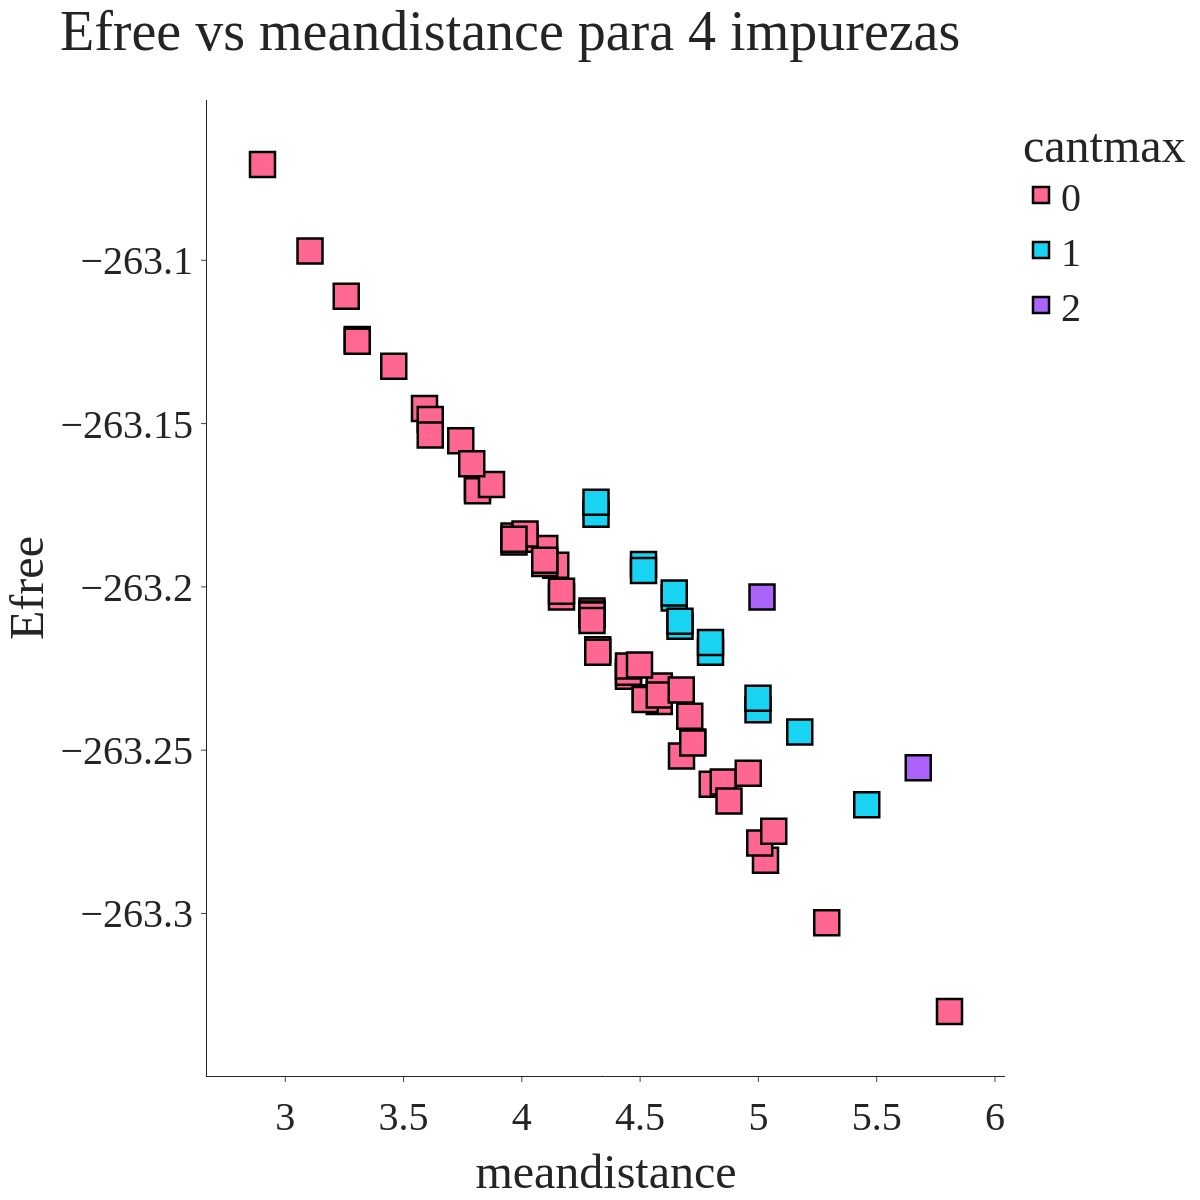
\includegraphics[width=\textwidth]{images/4_impurezas_cantmax_size10.png}
    \end{minipage}%
    \begin{minipage}[t]{0.5\textwidth}
        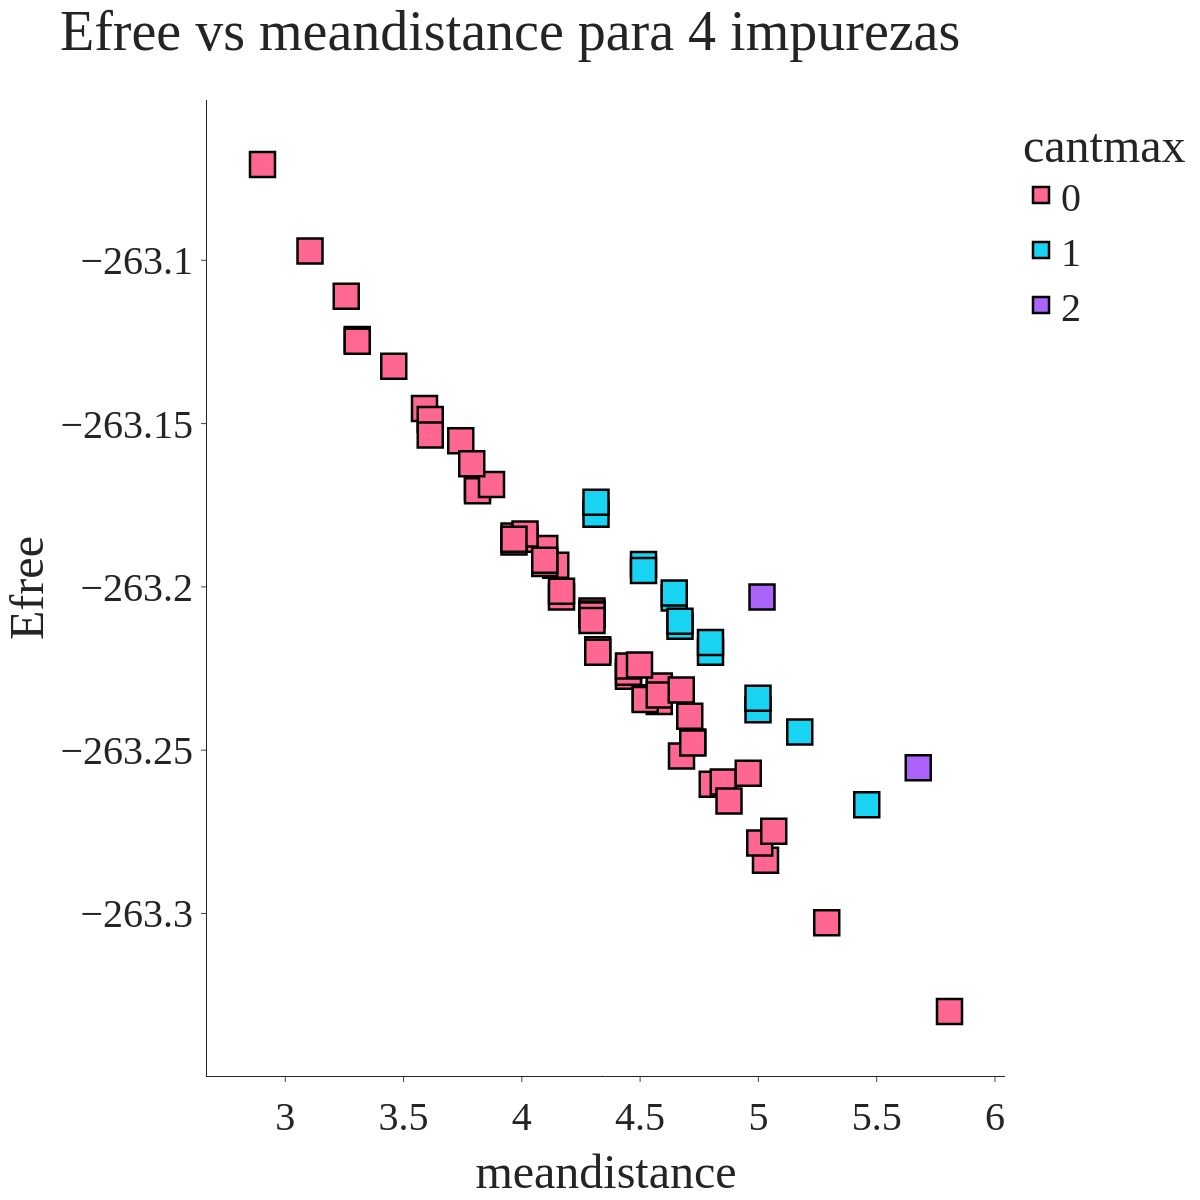
\includegraphics[width=\textwidth]{images/4_impurezas_cantmax_size10.png}    \end{minipage}%
    \caption{Ejemplo de scatterplot hecho con matplotlib.}
    \label{fig:scatterplot_3}
\end{figure}





\begin{mdframed}
    Recuerde que es imprescindible que se pueda replicar la generación de las gráficas, por lo que usted debe incluir cómo generó esos datos y  cómo podría generarlos la persona que revisa su entrega y ejecuta sus programas. Por ejemplo, si genera un scatterpolot con Tikz, usted debe explicar cómo obtener la tupla de valores que se usaron para generar la gráfica.
\end{mdframed}


\newpage
\section{Conclusiones}
\begin{mdframed}
    \textbf{La extensión máxima para esta sección es de 1 página.}
\end{mdframed}

La conclusión de su informe debe enfocarse en el resultado más importante de su trabajo. No se trata de repetir los puntos ya mencionados en el cuerpo del informe, sino de interpretar sus hallazgos desde un nivel más abstracto. En lugar de describir nuevamente lo que hizo, muestre cómo sus resultados responden a la necesidad planteada en la introducción.

\begin{itemize}
    \item  No vuelva a describir lo que ya explicó en el desarrollo del informe. En cambio, interprete sus resultados a un nivel superior, mostrando su relevancia y significado.
    \item Aunque no debe repetir la introducción, la conclusión debe mostrar hasta qué punto logró abordar el problema o necesidad planteada en el inicio. Reflexione sobre el éxito de su análisis o experimento en relación con los objetivos propuestos.
    \item No es necesario restablecer todo lo que hizo (ya lo ha explicado en las secciones anteriores). En su lugar, centre la conclusión en lo que significan sus resultados y cómo contribuyen al entendimiento del problema o tema abordado.
    \item No deben centrarse en sí mismos o en lo que hicieron durante el trabajo (por ejemplo, evitando frases como "primero hicimos esto, luego esto otro...").
    \item Lo más importante es que no se incluyan conclusiones que no se deriven directamente de los resultados obtenidos. Cada afirmación en la conclusión debe estar respaldada por el análisis o los datos presentados. Se debe evitar extraer conclusiones generales o excesivamente amplias que no puedan justificarse con los experimentos realizados.
\end{itemize}


\newpage



\printbibliography


\end{document}


